\chapter{Strumenti numerici indicatori - parte III}

\begin{figure}[h]
    \centering
    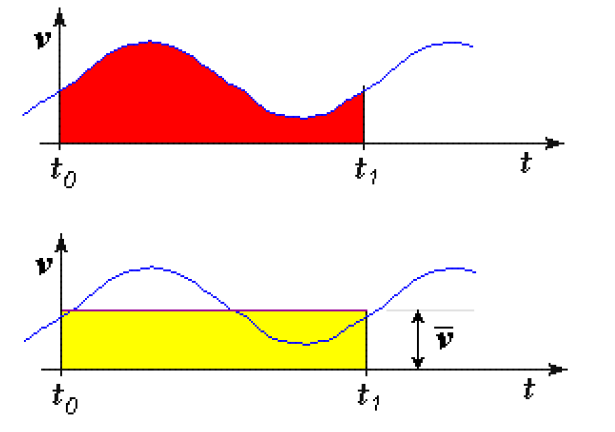
\includegraphics[scale = 1]{Da funzione istantanea analogica a valore medio.PNG}
\end{figure}

\newpage    

\section{Potenziale e tensione elettrica}
\footnote{Slide della prof | SDME 4 Strumenti numerici indicatori - parte III | pag 4 \\  
Appunti | 2025-04-29 | pag 7}

Prima di capire quali grandezze i multimetri misurano veramente, 
bisogna dare alcuni indicazioni e specificazioni riguardo alcuni termini. \newline 

Per potenziale elettrico in un punto si intende l'energia potenziale posseduta 
da una carica unitaria posta nel punto di cui si tratta e si esprime in joule / coulomb o volt: 

{
    \Large 
    \begin{equation}
        1 \text{ } J \cdot C^{-1} 
        = 
        1 \text{ } m^{2} \cdot kg \cdot s^{-3} \cdot A ^{-1} 
        = 
        1 \text{ } V
    \end{equation}
}

Per tensione elettrica fra due punti si intende la differenza dei loro potenziali elettrici. \newline 

La tensione elettrica viene chiamata anche differenza di potenziale. \newline 

\newpage 

\section{Corrente elettrica e sua intensità}
\footnote{Slide della prof | SDME 4 Strumenti numerici indicatori - parte III | pag 5 \\  
Appunti | 2025-04-29 | pag 7}

Per corrente elettrica si intende un flusso di particelle cariche o ioni. \newline 

Come studiato ad elettromagnetismo, per generare una corrente elettrica, si deve applicare un campo elettrico che muova 
le particelle cariche verso una direzione ben definita. \newline 

Invece, per intensità della corrente elettrica in un conduttore, si intende la carica elettrica che fluisce nella unità 
di tempo attraverso una sezione del conduttore stesso e si esprime in ampere, che è una u.d.m. di base dell'SI. \newline 

\newpage 

\section{Segnali elettrici (o no?): analisi o misurazione?}
\footnote{Slide della prof | SDME 4 Strumenti numerici indicatori - parte III | pag 6 - 7 \\  
Appunti | 2025-04-29 | pag 7 - 8}


La tensione e la corrente elettrica possono essere trattate come segnali, quando sono i veicoli di una informazione; 
oppure come generiche grandezze elettriche, quando ciò che interessa maggiormente è il trasferimento di energia, 
cioè non come abbiamo studiato i segnali nel corso di telecomunicazioni. \newline 

A seconda dei casi, delle generiche grandezze elettriche si esaminano gli andamenti temporali delle variazioni rispetto ad uno stato 
di riferimento: si tratta di analisi dei segnali, 
oppure si misureranno i valori di parametri descrittivi, cioè la misurazione delle grandezze elettriche  
(il focus di questo corso di misure elettriche ed elettroniche e non il focus del corso di telecomunicazioni). \newline 

Un esempio banale è quello delle grandezze elettriche in un proiettore: 

\begin{figure}[h]
    \centering
    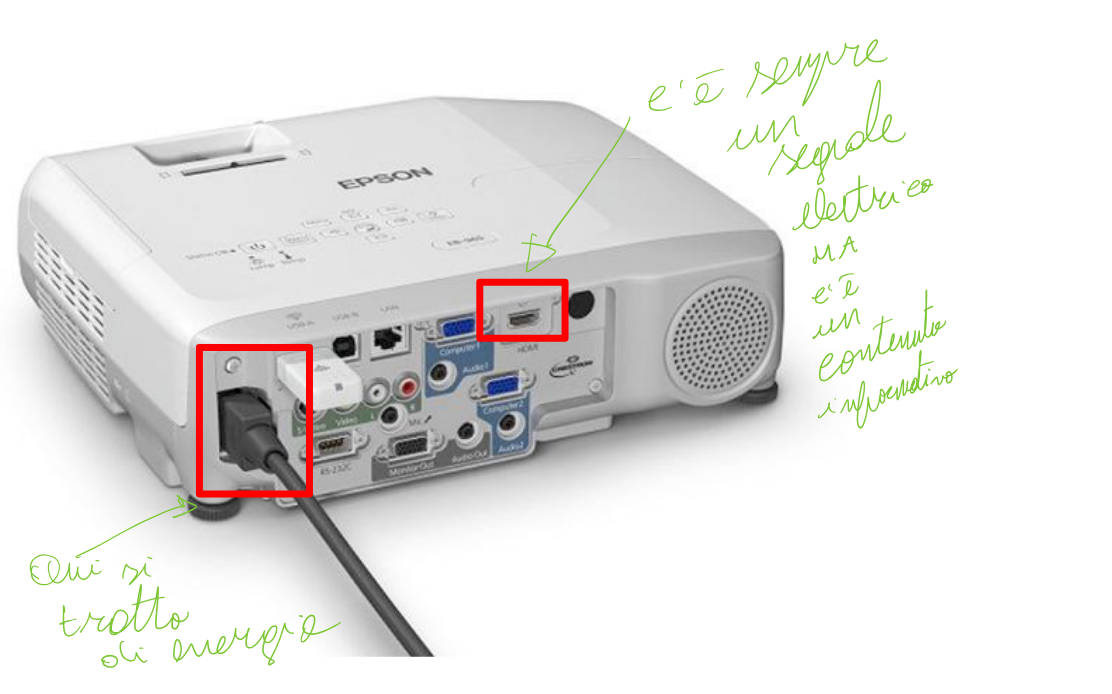
\includegraphics[scale = 0.8]{proiettore con annotazioni.PNG}
\end{figure}

\newpage 

\section{Il voltmetro misura la tensione ?}
\footnote{Slide della prof | SDME 4 Strumenti numerici indicatori - parte III | pag  8 - 9\\  
Appunti | 2025-04-29 | pag 9}

Come scritto precedentemente, il misurista esamina l'energia della grandezza fisica e non l'informazione come nel 
caso di un telecomunicazionista. \newline 

Ad esempio l'oscilloscopio è uno strumento che impiega sia il misurista che il telecomunicazionista nel proprio lavoro, 
ma l'oscilloscopio è uno strumento analizzatore, a differenza dei multimetri che misurano solo alcuni parametri descrittivi della grandezza fisica. \newline 

Come si può notare dalla figura dell'oscilloscopio: 

\begin{figure}[h]
    \centering
    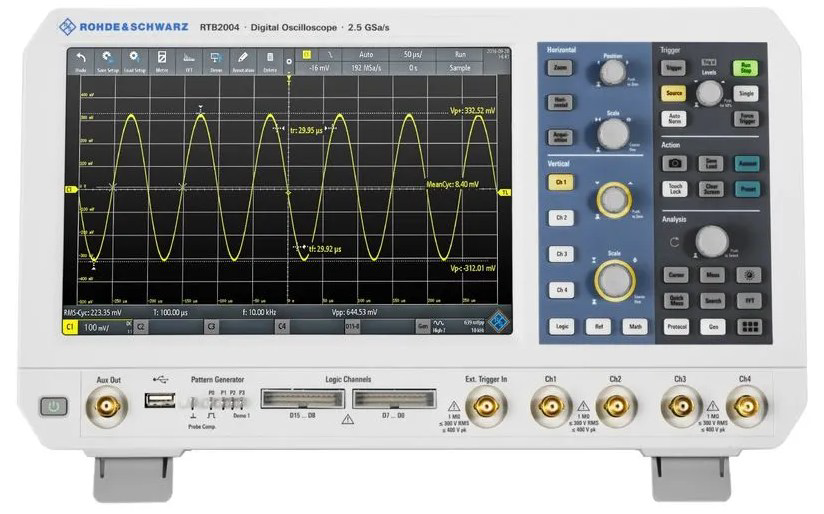
\includegraphics[scale = 0.8]{oscilloscopio.png}
\end{figure}

esso misura i valori istantanei. \newline 

Invece il voltmetro: 

\begin{figure}[h]
    \centering
    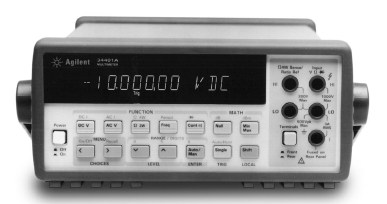
\includegraphics[scale = 1]{multimetro da banco.png}
\end{figure}

misura un valore medio stazionario, che è quello che interessa ad un misurista. \newline 


Oramai gli oscilloscopi moderni possono fare anche da multimetri, ma non sono i dispositivi più adatti. \newline 

\newpage 

\section{Parametri e parametri stazionari}
\footnote{Slide della prof | SDME 4 Strumenti numerici indicatori - parte III | pag  10 - 14\\  
Appunti | 2025-04-29 | pag 9 - 10}

Il parametro valore istantaneo v(t) all'istante $t_1$ 
rappresenta il valore assunto dalla tensione elettrica nell'istante $t = t_1$. \newline 

Il parametro valore istantaneo di corrente i(t) all'istante $t_1$ rappresenta 
il valore assunto dall'intensità della corrente elettrica nell'istante $t = t_1$, 
valore che è rappresentato dal rapporto fra la carica transitata in un intervallo di tempo infinitesimo centrato su $t_1$ 
e la durata, infinitesima, di tale intervallo. \newline 

Se si considera una funzione di questo tipo: 

\begin{figure}[h]
    \centering
    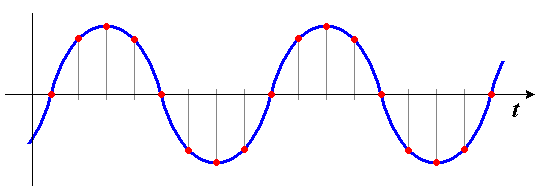
\includegraphics[scale = 1]{Frequenza di campionamento a 8B.png}
\end{figure}

in ogni pallino rosso è possibile definire il valore istantaneo della funzione v(t). \newline 

L'oscilloscopio è uno strumento che può misurare questi valori, 
a differenza del multimetro che può misurare solo il valore medio dato un intervallo di tempo. \newline 

Il parametro valore medio nell'intervallo $[t_0, t_1]$ rappresenta la media dei valori istantanei 
assunti dalla grandezza sotto misurazione nell'intervallo che inizia in $t_0$ e termina in $t_1$. \newline 

Se si considera una tensione v(t), si può definire il valore medio di questa tensione nell'intervallo $[t_0, t_1]$ come: 

{
    \Large 
    \begin{equation}
        \left. \overline{v} \right|_{[t_0, t_1]} 
        = 
        \frac{1}{t_1 - t_0}
        \int_{t_0}^{t_1} 
        v(t) dt
    \end{equation}
}


\begin{tcolorbox}
    La formula della media di una funzione è data dal teorema della media integrale. \newline 
    
    Se vuoi farti un piccolo ripasso: 

    Teorema della media integrale di Francesco Bigolin 

    \url{https://www.youtube.com/watch?v=N-GkcIlCyOo}

\end{tcolorbox}

Dalla formula di $ \left. \overline{v} \right|_{[t_0, t_1]}$ 
si può notare che v(t) può essere di qualsiasi valore nel tempo, periodica o non periodica: 
il valore medio dipende dall'intervallo scelto tra $[t_0, t_1]$. \newline 

\newpage 

Come si può visualizzare dalle seguenti figure: 

\begin{figure}[h]
    \centering
    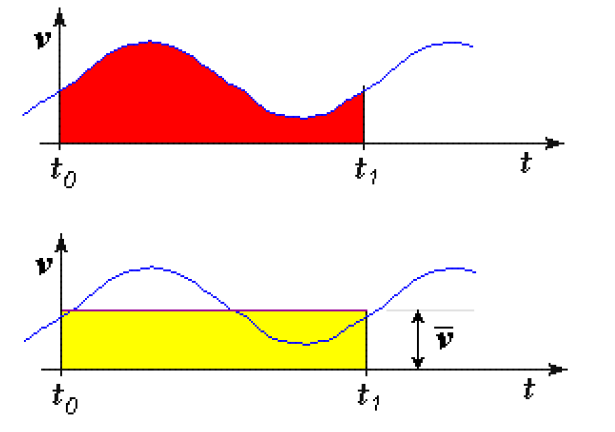
\includegraphics[scale = 0.8]{Da funzione istantanea analogica a valore medio.PNG}
\end{figure}



se si considera in rosso l'integrale della funzione v(t) nell'intervallo $[t_0, t_1]$, 
in cui v(t) varia istantaneamente, 
in giallo è indicato il valore medio di v(t) in quell'intervallo. \newline 

$ \left. \overline{v} \right|_{[t_0, t_1]}$ può essere vista come una funzione continua costante in quell'intervallo. \newline 

È anche definito il valore medio della corrente nell'intervallo $[t_0, t_1]$ come: 

{
    \Large 
    \begin{equation}
        \left. \overline{i} \right|_{[t_0, t_1]} 
        = 
        \frac{1}{t_1 - t_0}
        \int_{t_0}^{t_1} 
        i(t) dt
    \end{equation}
}

\newpage 

\section{Valore efficace}
\footnote{Slide della prof | SDME 4 Strumenti numerici indicatori - parte III | pag  15, 23 \\  
Appunti | 2025-04-29 | pag 10} 

Un altro parametro molto importante è il valore efficace. \newline 

In un tempo pari ad un periodo T, una corrente alternata con valore efficace di 1 A che circola su di un resistore 
dissipa la stessa energia che sarebbe dissipata nello stesso tempo, da una corrente costante con intensità di 1 A. \newline 

Per dare questa definizione, la corrente alternata è periodica ed ha valore medio nullo. \newline 

In formule: 

{
    \Large 
    \begin{equation}
        I 
        = 
        \sqrt
        {
            \frac{1}{T}
            \int_{t_0}^{t_0 + T} 
            i^{2} (t) dt
        }
    \end{equation}
}

Anche se fisicamente non esiste, 
si è data anche la definizione di tensione efficace come: 

{
    \Large 
    \begin{equation}
        V 
        = 
        \sqrt
        {
            \frac{1}{T}
            \int_{t_0}^{t_0 + T} 
            v^{2} (t) dt
        }
    \end{equation}
}

\begin{tcolorbox}
Stare attenti alla nomenclatura: I e V con le lettere maiuscole intendono rispettivamente la corrente efficace e la tensione efficace    
\end{tcolorbox}

\newpage 

\subsection{Perché dalla distribuzione in continua si è passati alla alternata}
\footnote{Slide della prof | SDME 4 Strumenti numerici indicatori - parte III | pag  16 - 22 \\  
Appunti | 2025-04-29 | pag 10} 

\begin{tcolorbox}
    Momento storico alla Piero Angela pag 16 - 18 

    Se volete approfondire: 

    \url{https://www.storiadimilano.it/citta/milanotecnica/elettricita/radegonda0.htm}
\end{tcolorbox}

In breve, si è passati da una distribuzione di corrente continua ad alternata perchè la dissipazione in continua in lunghe tratte è enorme. \newline 

Se si considera la funzione della corrente sinusoidale (consideriamola idealmente sinusoidale e con un'unica pulsazione $\omega$, anche se nella realtà non è così): 

{
    \Large 
    \begin{equation}
        i(t) = I_{pk} \cdot \sin(\omega t)
    \end{equation}
} 

dove $I_{pk}$ è la corrente di picco, possiamo calcolarci la corrente efficace I come: 

{
    \Large 
    \begin{equation}
        \begin{split}
        I 
        &= 
        \sqrt
        {
            \frac{1}{T}
            \int_{t_0}^{t_0 + T} 
            i^{2} (t) dt
        }
        \\ 
        &=
        \sqrt
        {
            \frac{1}{T}
            \int_{t_0}^{t_0 + T} 
            \left[I_{pk} \cdot \sin(\omega t) \right] ^{2} 
            dt
        } 
        \\ 
        &=
        \sqrt
        {
            \frac{I_{pk}^{2}}{T}
            \int_{t_0}^{t_0 + T} 
            \left[ \sin(\omega t) \right] ^{2} 
            dt
        }  
        \end{split}
    \end{equation}
}

Grazie alle identità trigonometriche, possiamo scrivere $\left[ \sin(\omega t) \right] ^{2} $ come: 

{
    \Large 
    \begin{equation}
        \begin{split}
        &= 
        \sqrt
        {
            \frac{I_{pk}^{2}}{T}
            \int_{t_0}^{t_0 + T}
            \frac{1 - \cos(2 \omega t)}{2} 
            dt
        }
        \\
        &= 
        \sqrt
        {
            \frac{I_{pk}^{2}}{T}
            \left[ 
            \int_{t_0}^{t_0 + T}
            \frac{1}{2} 
            dt
            +
            \int_{t_0}^{t_0 + T}
            \frac{-\cos(2 \omega t)}{2} 
            dt
            \right]
        }
        \end{split}
    \end{equation}
}

Se si considera una sinusoide ideale a valore medio nullo, 
il secondo integrale è nullo, quindi: 

{
    \Large 
    \begin{equation}
        \begin{split}
         &= 
        \sqrt
        {
            \frac{I_{pk}^{2}}{T}
            \left[ 
            \int_{t_0}^{t_0 + T}
            \frac{1}{2} 
            dt
            +
            0
            \right]
        }
        \\ 
        &= 
        \sqrt
        {
            \frac{I_{pk}^{2}}{T}
            \int_{t_0}^{t_0 + T}
            \frac{1}{2} 
            dt
        }
        \\
        &=
        \sqrt
        {
            \frac{I_{pk}^{2}}{T}
            \cdot
            \frac{1}{2} 
            T 
        }
        \\
        &= 
        \sqrt{\frac{I_{pk} ^{2}}{2}}
        \\ 
        &= 
        \frac{I_{pk}}{\sqrt{2}}
        \end{split}
    \end{equation}
}

Con questa dimostrazione, si può dire che si può calcolare il RMS (Root Mean Square), 
cioè il valore efficace di un segnale come: 

{
    \Large 
    \begin{equation}
        I = \frac{I_{pk}}{\sqrt{2}}
    \end{equation}
}

Questo calcolo, come vedremo in seguito, può essere dato o a un dispositivo DSP che esegue questo calcolo numerico oppure ad un circuito. \newline 

Se invece si applica la formula dell'integrale del valore efficace I, 
si definisce il segnale I come TRMS (True Root Mean Square). \newline 

Se i segnali sono perfettamente sinusoidali: 

{
    \Large 
    \begin{equation}
        RMS = TRMS
    \end{equation}
}

ma in generale non lo sono. \newline 

\newpage

\section{Il multimetro numerico}
\footnote{Slide della prof | SDME 4 Strumenti numerici indicatori - parte III | pag  24 \\  
Appunti | 2025-04-29 | pag 4} 

Come scritto precedentemente, 
uno strumento di misura numerico ha molteplici vantaggi, tra cui può svolgere da voltmetro numerico. \newline 

\begin{tcolorbox}
    Si scrive voltmetro, non voltimetro, voltometro. \newline 
    Voltmetro, fine della discussione. Baci baci \newline 

    Se ancora non lo capisci, fattelo dire da Shrek: \\
    \url{https://www.youtube.com/watch?v=YK8OEdhu-1c} minuto 1:40 - 1:45
\end{tcolorbox}

Nel corso andremo a studiare le seguente funzioni del voltmetro numerico a valore medio: 

\begin{itemize}
    \item lo schema elettrico di principio 
    \item la misurazione del valore medio, quindi attenuazione dei disturbi e la scelta del periodo di mediazione 
    \item il partitore di ingresso 
    \item la protezione contro le sovratensione dell'ingresso (caratteristica molto importante in un qualsiasi strumento di misura) 
    \item il convertitore AD a valore medio 
\end{itemize}

\newpage 

\subsection{Funzioni del multimetro}
\footnote{Slide della prof | SDME 4 Strumenti numerici indicatori - parte III | pag  25 \\  
Appunti | 2025-04-30 | pag 4} 

I multimetri, chiamati anche come "tester", misurano più di una grandezza elettrica. \newline 

Di seguito le specifiche di un Fluke 112: 

\begin{figure}[h]
    \centering
    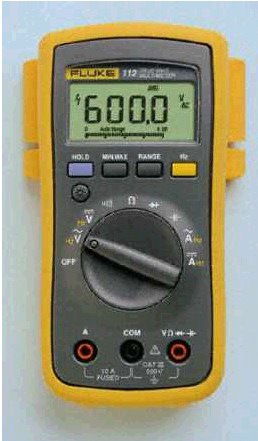
\includegraphics[scale = 0.5]{Fluke 112.png}
    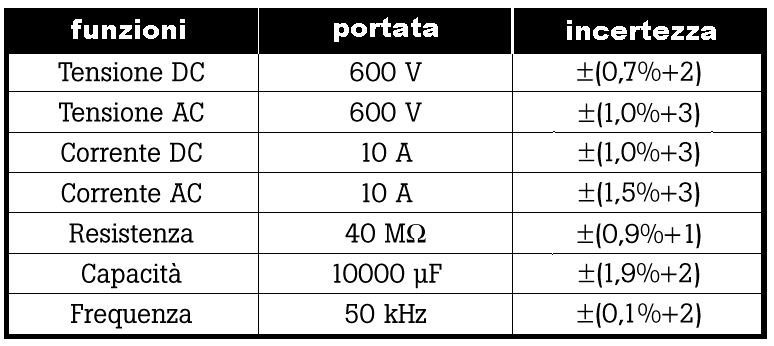
\includegraphics[scale = 0.8]{Specifiche Fluke 112.png }
\end{figure}

Come si può visualizzare dalla tabella, il tester fa lo stesso ruolo di: 

\begin{itemize}
    \item voltmetro, quindi misura una tensione 
    \item amperometro, quindi misura una corrente 
    \item Ohmetro, quindi misura una resistenza
\end{itemize}

La corrente e la tensione possono essere alternate (AC) o non alternate (DC). \newline 

\newpage 

\subsection{Gli "strumenti elementari" che costituiscono il multimetro numerico}
\footnote{Slide della prof | SDME 4 Strumenti numerici indicatori - parte III | pag  26 \\  
Appunti | 2025-04-30 | pag 4} 

Come scritto precedentemente, il tester comprende più strumenti in uno. \newline 

In particolare: 

\begin{itemize}
    \item nel voltmetro si può svolgere una misura del valore medio e del valore efficace della tensione 
    \item nell'amperometro si può svolgere una misura del valore medio e del valore efficace dell'intensità di corrente
\end{itemize}

\newpage 

\section{Il voltmetro a valore medio}
\footnote{Slide della prof | SDME 4 Strumenti numerici indicatori - parte III | pag  27-28 \\  
Appunti | 2025-04-29 | pag 4} 

Di seguito una rappresentazione dell'architettura di un voltmetro a valore medio: 

\begin{figure}[h]
    \centering
    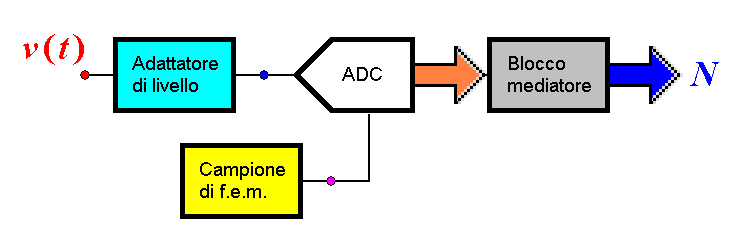
\includegraphics[scale = 1]{schema volmetro a valore medio.png}
\end{figure} 

Come visualizzato nello schema, i componenti principali di un voltmetro a valore medio sono: 

\begin{itemize}
    \item uno stadio di ingresso (blocco celestino "Adattatore di livello") con protezioni contro le sovratensioni e adattatore di livello, che, nell'architettura del voltmetro, adatta, generalmente, una alta tensione in piccole tensioni che lo strumento numerico può gestire
    \item un campione di f.e.m. (blocco giallo), che generalmente servirà come riferimento all'ADC 
    \item un convertitore AD (pentagono bianco ADC), che è il componente più importante, più costoso, più delicato di tutta l'architettura (praticamente da accudire come Biancaneve) 
    \item generalmente, un display per visualizzare la misura 
\end{itemize}

A sua volta, si può considerare l'architettura del voltmetro numerico a valore medio in due parti: 

\begin{itemize}
    \item circuito analogico, che comprende lo stadio di ingresso, campione di f.e.m. e lo stadio di ingresso dell'ADC 
    \item circuito digitale, che comprende lo stadio di uscita dell'ADC, il blocco mediatore e il display
\end{itemize}

È consuetudine rappresentare l'architettura del voltmetro a valore medio con questa rappresentazione: 

\begin{figure}[h]
    \centering
    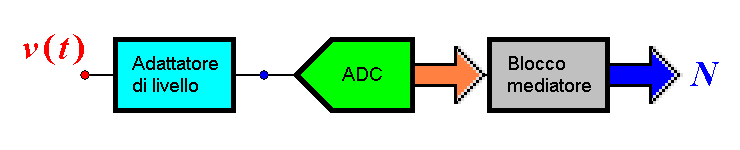
\includegraphics[scale = 1]{schema volmetro a valore medio schema usuale.png}
\end{figure} 

Il campione di f.e.m. è generalmente inglobato nell'architettura dell'ADC ed è realizzato con il silicio con un diodo zener. \newline 

Inoltre, N, cioè il valore di misura che uscirà dal circuito sarà: 

{
    \Large 
    \begin{equation}
        N 
        = 
        \alpha 
        \left.
        \overline{v_x}
        \right|_{[t_0, t_1]}
    \end{equation}
}

dove: 

\begin{itemize}
    \item $\left. \overline{v_x} \right|_{[t_0, t_1]}$ è la tensione media di ingresso v(t) (che può essere sia periodica che non periodica, che sinusoidale che non sinusoidale) calcolata nell'intervallo $[t_0, t_1]$
    \item $\alpha$ è la costante di taratura (idealmente $\alpha = 1$), che è proporzionale a $\left. \overline{v_x} \right|_{[t_0, t_1]}$
\end{itemize}

Ora ci concentreremo su come scegliere l'intervallo di tempo $[t_0, t_1]$ e come realizzare il blocco mediatore. \newline 

\newpage 

\subsection{Perché usare uno strumento a valore medio?}
\footnote{Slide della prof | SDME 4 Strumenti numerici indicatori - parte III | pag  29 \\  
Appunti | 2025-04-30 | pag 5} 

Consideriamo, come esempio, il segnale elettrico di una termocoppia, cioè uno strumento che "converte" una temperatura $\theta$ 
in una tensione v come uscita: 

\begin{figure}[h]
    \centering
    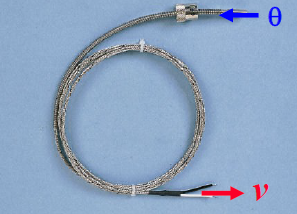
\includegraphics[scale = 1]{Termocoppia.PNG}
\end{figure} 

Se si considera l'andamento nel tempo da un punto di vista macro: 

\begin{figure}[h]
    \centering
    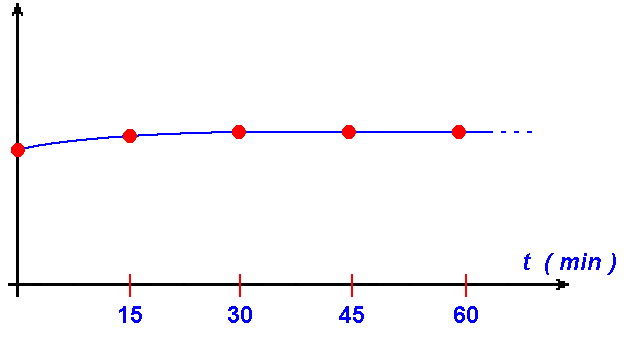
\includegraphics[scale = 1]{Valori termocoppia nel tempo.png}
\end{figure} 

Da un punto di vista micro, "facendo uno zoom" su un pallino rosso, notiamo che: 

\begin{figure}[h]
    \centering
    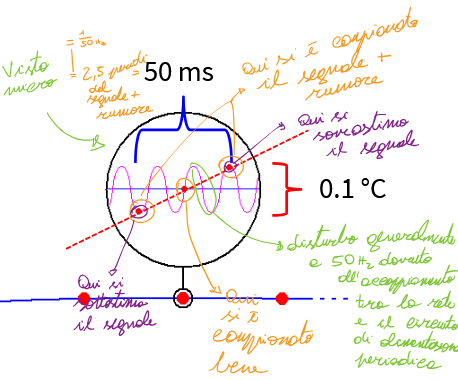
\includegraphics[scale = 1.2]{Valori termocoppia nel tempo zoom con note.png}
\end{figure} 

Generalmente, anche se casuale, il disturbo è più piccolo rispetto al segnale utile. \newline 

Si può tecnicamente misurare la tensione istantanea, ma non avrebbe senso dal punto di vista misuristico perchè 
la media attenua gli effetti casuali della singola ripetizione. \newline 

La media va fatto su un periodo ben fissato: è il disturbo che impone la durata in cui fare la media. \newline 

Siccome, in Europa, molti dispositivi soffrono di disturbi dovuti 
alla rete di distribuzione elettrica, la quale eroga corrente a 50 Hz: 

{
    \Large 
    \begin{equation}
        \begin{split}
        50 \text{ } Hz 
        &= 
        \frac{1}{50} \text{ } s
        \\ 
        &= 
        0.02 \text{ } s
        \\ 
        &= 
        20 \text{ } ms
        \end{split}
    \end{equation}
}

si cerca di scegliere un intervallo per calcolare il valore medio della tensione 
un multiplo di tale disturbo, cioè 50 ms, che è 2.5 il disturbo della rete di distribuzione di 20 ms. \newline 

\newpage 

\subsection{Cancellazione di un rumore alternato}
\footnote{Slide della prof | SDME 4 Strumenti numerici indicatori - parte III | pag  30 \\  
Appunti | 2025-04-29 | pag 6} 

Una grandezze si dice alternata se il suo valore medio sul periodo è nulla. \newline 

Un rumore alternato è quindi periodico ed ha, sul periodo, un valore medio nullo. \newline 

Consideriamo un segnale s sommato al rumore r e calcoliamone il suo valore medio nell'intervallo $[t_0, t_1]$: 

{
    \Large
    \begin{equation}
        \begin{split}
        \overline{s + r}
        &= 
        \frac{1}{t_1 - t_0}
        \int_{t_0}^{t_1}
        \left[ 
            s(t) + r(t)
        \right]
        dt
        \\
        &= 
        \frac{1}{t_1 - t_0}
        \int_{t_0}^{t_1}
            s(t)
        dt 
        +
        \frac{1}{t_1 - t_0}
        \int_{t_0}^{t_1}
            r(t)
        dt
        \end{split}
    \end{equation}
}

Supponiamo che il rumore sia additivo, cioè r rumore si sommi al segnale sotto misura s. \newline 

Se si sceglie un intervallo del disturbo alternato $T_r$: 

{
    \Large 
    \begin{equation}
        T_r = t_1 - t_0
    \end{equation}
} 

allora l'equazione di $\overline{s + r}$ diventa: 

{
    \Large 
    \begin{equation}
        \begin{split}
        \overline{s + r}
        &= 
        \frac{1}{t_1 - t_0}
        \int_{t_0}^{t_1}
            s(t)
        dt 
        +
        0
        \\ 
        &= 
        \frac{1}{t_1 - t_0}
        \int_{t_0}^{t_1}
            s(t)
        dt
        \\ 
        &= 
        \overline{s}           
        \end{split}
    \end{equation}
}

Questa ultima equazione, cioè che: 

{
    \Large 
    \begin{equation}
        \overline{s + r}
        = 
        \overline{s}
    \end{equation}
}

ci permette di dire che, se il rumore entra dentro il circuito del voltmetro, 
non c'è bisogno di inserire un blocco filtrante per togliere il rumore, 
proprio perchè il rumore, nel periodo $T_r$, ha valore medio nullo. \newline 

\newpage 

\subsection{Cancellazione di un rumore alternato tramite misurazione del valore medio}
\footnote{Slide della prof | SDME 4 Strumenti numerici indicatori - parte III | pag  31 \\  
Appunti | 2025-04-30 | pag 6} 

Considerando il seguente segnale sommato ad un rumore con andamento alternato, il suo andamento macroscopico rispetto all'andamento microscopico sarà: 

\begin{figure}[h]
    \centering
    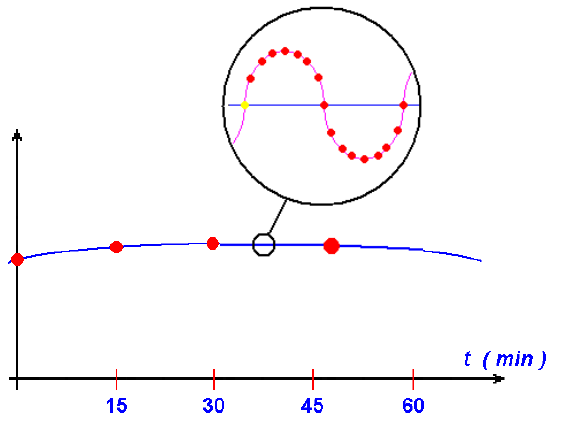
\includegraphics[scale = 1]{Andamento microscopico e macroscopico di un segnale.PNG}
\end{figure} 

Con le considerazioni svolte precedentemente, possiamo scrivere che, se s è il segnale ed r è il rumore alternato: 

{
    \Large 
    \begin{equation}
        \begin{split}
            \overline{s + r} 
            &=
            \frac{1}{K}
            \sum_{j = 1}^{K}
            \left[ 
                s (t_j) + r(t_j)
            \right] 
            \\
            &= 
            \frac{1}{K}
            \sum_{j = 1}^{K}
            \left[ 
                s (t_j) 
            \right] 
            + 
            \frac{1}{K}
            \sum_{j = 1}^{K}
            \left[
            r(t_j)
            \right]
            \\
            &= 
            \frac{1}{K}
            \sum_{j = 1}^{K}
            \left[ 
                s (t_j) 
            \right] 
            + 
            0
            \\ 
            &= 
            \frac{1}{K}
            \sum_{j = 1}^{K}
            \left[ 
                s (t_j) 
            \right] 
            \\ 
            &= 
            \overline{s}
        \end{split}
    \end{equation}
}

in cui $\overline{s}$ è la media del segnale s nel periodo $T_r$:

{
    \Large 
    \begin{equation}
        \begin{cases}
            t_j = t_0 + j \frac{T_r}{K}
            \\ 
            K \in \mathbb{Z} 
        \end{cases}
    \end{equation}
}

K è il numero di valori istantanei misurati all'interno di quello che è il periodo del rumore $T_r$, 
prendendo valori equi-spaziati che coprono un intero periodo. \newline 

Come scritto nella sezione precedente, non è necessario un blocco filtrante per togliere il rumore, 
se questo ultimo è alternato e periodico. \newline 

\newpage 

\section{Media numerico o analogica?}
\footnote{Slide della prof | SDME 4 Strumenti numerici indicatori - parte III | pag  32 \\  
Appunti | 2025-04-30 | pag 6}

Come possiamo notare dai seguenti modelli di multimetri da banco e dai loro rispettivi prezzi:

\begin{figure}[h]
    \centering
    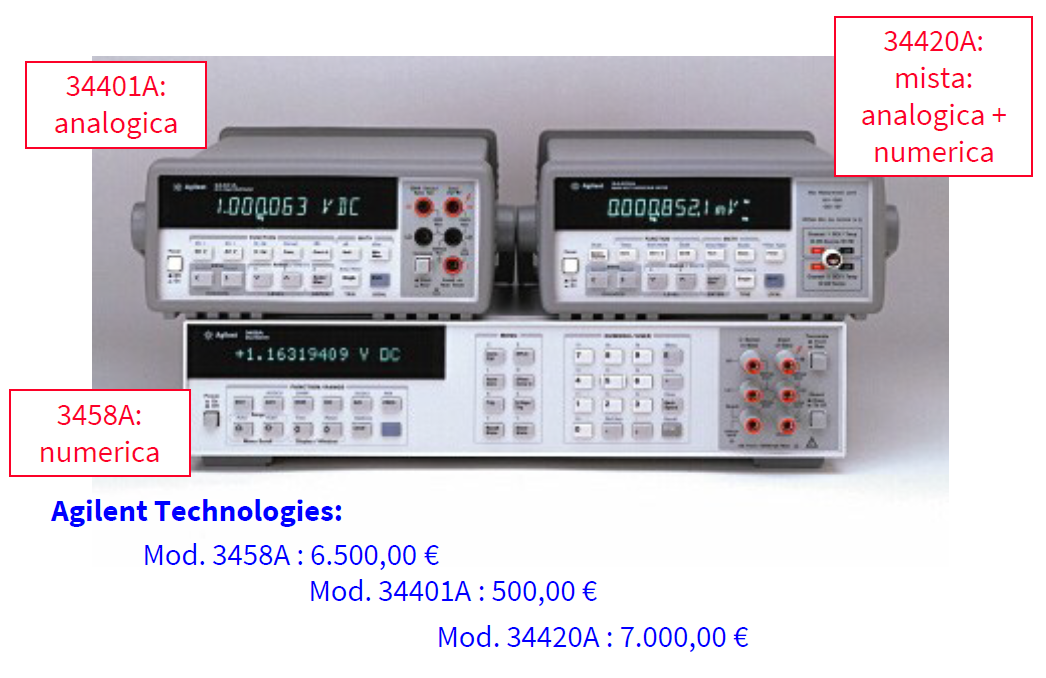
\includegraphics[scale = 0.8]{Confronto di costi tra multimetri.PNG}
\end{figure} 

Un approccio misto tra analogico e numerico del calcolo di una media del segnale ha un costo a livello economico più elevato 
perchè è più complesso da gestire, ma garantirà una minore incertezza di misura. \newline 

La stessa misura va svolta su due circuiti differenti e poi confrontati. \newline 

\newpage 

\subsection{Il voltmetro a valore medio: media numerica}
\footnote{Slide della prof | SDME 4 Strumenti numerici indicatori - parte III | pag  33\\  
Appunti | 2025-04-30 | pag 6}

Considerando il circuito all'interno di un voltmetro numerico: 

\begin{figure}[h]
    \centering
    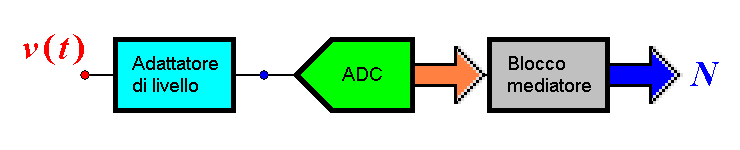
\includegraphics[scale = 1]{schema volmetro a valore medio schema usuale.png}
\end{figure} 

e l'andamento del segnale originale analogico e dei valori istantanei (pallini rossi in figura) nel periodo $[t_0, t_1]$: 

\begin{figure}[h]
    \centering
    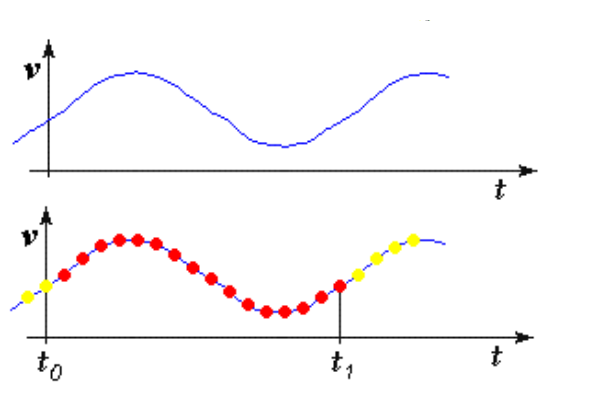
\includegraphics[scale = 0.8]{segnale analogico e valori istantanei.PNG}
\end{figure}

Se il voltmetro svolge una media numerica, il blocco mediatore, che è posto dopo l'ADC, 
svolge la seguente operazione matematica: 

{
    \Large 
    \begin{equation}
            \overline{v} = \frac{1}{K} \sum_{j = 1}^{K} \left[ v(t_j) \right]
    \end{equation}
}

in cui $t_j$ è preso come: 

{
    \Large 
    \begin{equation}
        t_j = t_0 + j \frac{t_1 - t_0}{K}
    \end{equation}
}

Siccome la media del segnale v viene svolta nel periodo $[t_0, t_1]$, 
possiamo scrivere: 

{
    \Large 
    \begin{equation}
        \overline{v} = \left. \overline{v_x} \right|_{[t_0, t_1]}
    \end{equation}
}

Il blocco mediatore da in uscita il valore N della misura che è uguale a: 

{
    \Large 
    \begin{equation}
        N = \alpha \left. \overline{v_x} \right|_{[t_0, t_1]}
    \end{equation}
}

dove $\alpha$ è la costante di taratura, 
che è proporzionale a $\left. \overline{v_x} \right|_{[t_0, t_1]}$. \newline 

\newpage 

\subsection{Il voltmetro a valore medio: integrazione analogica}
\footnote{Slide della prof | SDME 4 Strumenti numerici indicatori - parte III | pag  34\\  
Appunti | 2025-04-30 | pag 6}

Se invece si considera un volmetro che ha la seguente architettura: 

\begin{figure}[h]
    \centering
    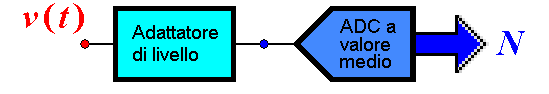
\includegraphics[scale = 1]{integrazione analogica voltmetro a valore medio.png}
\end{figure}

L'adattatore di livello diminuisce il segnale v(t), in modo che l'ADC a valore medio possa svolgere le sue operazioni. \newline 

Nel blocco (di colore blu) l'ADC a valore medio, 
è incluso il blocco integratore che svolge la seguente operazione: 

{
    \Large 
    \begin{equation}
    \left. \overline{v_x} \right|_{[t_0, t_1]}
    = 
    \frac{1}{t_1 - t_0}
    \int_{t_0}^{t_1}
    v(t) dt
    \end{equation}
}

cioè dal segnale analogico, si calcola l'integrale (banalmente l'area sotto al segnale):   

\begin{figure}[h]
    \centering
    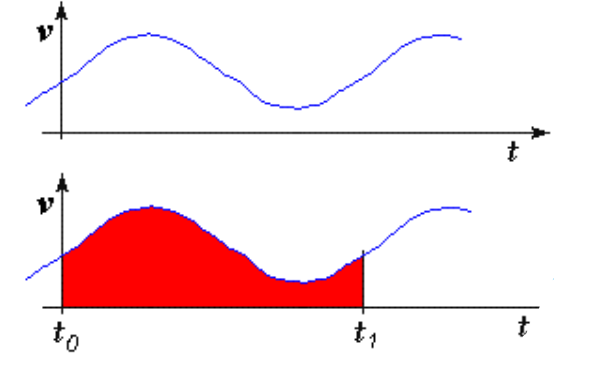
\includegraphics[scale = 1]{Integrale di un segnale analogico.PNG}
\end{figure}

(di colore rosso in figura) nel periodo $[t_0, t_1]$ e poi si fa la media. \newline 

N, come il caso del voltmetro in cui si svolge una media numerica, sarà: 

{
    \Large 
    \begin{equation}
        N = \alpha \left. \overline{v_x} \right|_{[t_0, t_1]}
    \end{equation}
}

ma in questo caso, rispetto al caso precedente, la media del segnale v(t) viene calcolata in modo analogico e non in modo numerico. \newline 

\newpage 

\section{Scelta dell'intervallo di media: spettro del rumore elettrico}
\footnote{Slide della prof | SDME 4 Strumenti numerici indicatori - parte III | pag  35 - 37\\  
Appunti | 2025-04-30 | pag 6 - 7}

Come visualizzato nei capitoli precedenti:  

\begin{figure}[h]
    \centering
    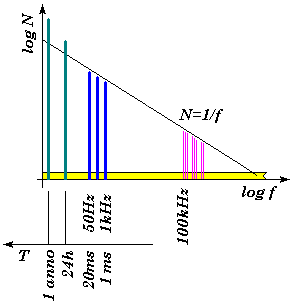
\includegraphics[scale = 1]{Disturbi elettromagnetici in base alla frequenza.png}
\end{figure}

l'entità del disturbo dipende dalla frequenza del segnale che dobbiamo analizzare. \newline 

Per scegliere l'intervallo sul quale effettuare la media, riconsideriamo lo spettro del rumore elettrico. \newline 

Non possiamo cancellare il rumore dovuto alle derive termiche, quelle a bassissima frequenza (quelle minori a 50 Hz). \newline 

Possiamo, però, cancellare i disturbi generati dalla rete a 50 Hz e quelli a frequenze superiori. \newline 

\begin{tcolorbox}
    In linea di massima, le frequenze basse sono quelle che interessano all'ambito elettrico; 
    invece le frequenze alte sono quelle che interessano l'ambito dell'elettronica
\end{tcolorbox}

Consideriamo l'andamento dei due segnali: 

\begin{figure}[h]
    \centering
    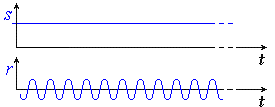
\includegraphics[scale = 2]{segnale di tensione e rumore.png}
\end{figure}

Il segnale s è la tensione da misurare, che rimane costante; 
invece r è il rumore a 50 Hz dovuto alla linea elettrica e lo consideriamo perfettamente sinusoidale e periodico. \newline  

Si vuole calcolare la media del segnale $\overline{s + r}$ in un periodo T. \newline 

Se il periodo T è proprio: 

{
    \Large 
    \begin{equation}
        T = [t_0, t_1]
    \end{equation}
}

che coincide con un periodo del segnale di rumore alternato, 
allora il valore medio del rumore sull'intervallo risulta nullo. \newline 

Come si può visualizzare dalla seguente figura: 

\begin{figure}[h]
    \centering
    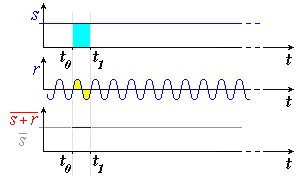
\includegraphics[scale = 2]{segnale di tensione e rumore calcolo media in un periodo.png}
\end{figure}

Il valore di $\overline{s+r}$ è uguale al valore medio di $\overline{s}$: essendo s costante, anche il valore medio di s, cioè $\overline{s}$, 
sono uguali. \newline 

Se si considera un periodo T più lungo, multiplo di $[t_0, t_1]$, ad esempio due volte $[t_0, t_1]$:

\begin{figure}[h]
    \centering
    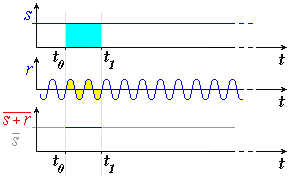
\includegraphics[scale = 2]{segnale di tensione e rumore calcolo media in due periodi.png}
\end{figure}

l'andamento di $\overline{s + r}$ rimane lo stesso di un periodo. \newline 

In generale, tutte le volte che l'intervallo è un multiplo intero del periodo del rumore, si riesce a cancellare il contributo di rumore. \newline 

\newpage 


Se l'intervallo $[t_0, t_1]$ non ha durata pari ad un multiplo intero del periodo di rumore, 
come in questo caso: 

\begin{figure}[h]
    \centering
    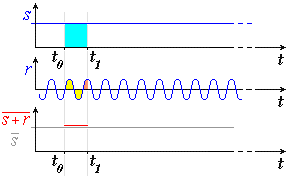
\includegraphics[scale = 2]{segnale di tensione e rumore calcolo media in un periodo e frazione.png}
\end{figure}

la semi-onda che non si elide, fornisce un piccolo contributo (nella figura di colore rosa carne) al valore medio. \newline 

La semi-onda in rosa carne viene "spalmata" sull'intervallo e dà un piccolo contributo a $\overline{s + r}$. \newline 

Quindi: 

{
    \Large 
    \begin{equation}
        \overline{s + r} \neq \overline{s}
    \end{equation}
}

Se consideriamo la condizione peggiore, cioè quando viene preso un intervallo $[t_0, t_1]$ 
proprio lungo una semi-onda del rumore: 

\begin{figure}[h]
    \centering
    \includegraphics[scale = 2]{segnale di tensione e rumore calcolo media in metà periodo.png}
\end{figure}

il contributo, che non si elide, porta ad un forte incremento del valore medio del segnale+rumore $\overline{s + r}$, 
rispetto al valore medio del solo segnale. \newline 

Però, prendendo un intervallo più lungo rispetto a $[t_0, t_1]$, 
il contributo di quella semi-onda di rumore si "spalma" su un tempo via via maggiore e diventa meno significativo. \newline 

\newpage 

Come si può visualizzare dalle seguenti figure, se si aumenta il tempo $[t_0, t_1]$ (confronta le figure da sinistra verso destra): 

\begin{figure}[h]
    \centering
    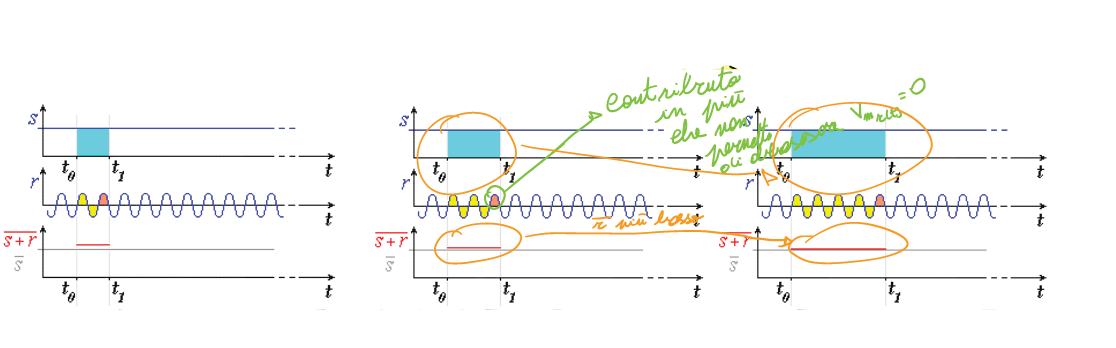
\includegraphics[scale = 0.8]{segnale di tensione e rumore calcolo media aumentando il periodo di misura.png}
\end{figure}

si può concludere che, più è lungo l'intervallo di misura rispetto al periodo del rumore, tanto minore sarà il residuo di alterazione che potrò trovare nella misura. \newline 

\newpage 

\section{Scelta dell'intervallo di media: reiezione rumori alternati}
\footnote{Slide della prof | SDME 4 Strumenti numerici indicatori - parte III | pag 38 \\  
Appunti | 2025-04-29 | pag 7}

Data il seguente grafico: 

\begin{figure}[h]
    \centering
    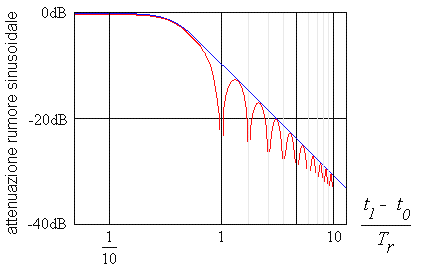
\includegraphics[scale = 2]{Reiezione dei rumori alternati rispetto alla durata di misura.png}
\end{figure}

si può dimostrare la reiezione dei rumori alternati in funzione del rapporto tra la durata dell'intervallo di tempo $t_1 - t_0$ sul quale si calcola la media 
e il periodo di rumore $T_r$. \newline 

Tutte le volte che il rapporto è un intero, si ha un'attenuazione totale del rumore: 
alche nella figura l'andamento rosso non ha un valore. \newline 

Quando non sussiste questa condizione, il residuo di rumore diminuisce quanto più l'intervallo $t_1 - t_0$ è maggiore di $T_r$. \newline 

Si ha dunque interesse a prendere intervalli lunghi, ma c'è un problema dovuto al residuo di rete. \newline 

\newpage 

\section{Scelta dell'intervallo di media: "residuo di rete"}
\footnote{Slide della prof | SDME 4 Strumenti numerici indicatori - parte III | pag 39 \\  
Appunti | 2025-04-29 | pag 7}

La rete elettrica ha un andamento (idealmente) sinusoidale di una frequenza nota. \newline 

In Europa, la rete elettrica distribuisce tensione a 50 Hz, quindi il periodo del disturbo è: 

{
    \Large 
    \begin{equation}
        \begin{split}
            f_{rE} = 50 \text{ Hz } 
            \leftrightarrow 
            T_{rE} 
            &=  \frac{1}{f_{rE}}
            \\
            &= \frac{1}{50} \text{ s }
            \\ 
            &= 20 \text{ ms}
        \end{split}
    \end{equation}
}

Con l'aiuto della seguente figura: 

\begin{figure}[h]
    \centering
    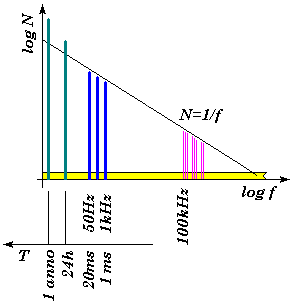
\includegraphics[scale = 1]{Disturbi elettromagnetici in base alla frequenza.png}
\end{figure}

e dal corso di Teoria dei Segnali (o Segnali Determinati Aleatori), 
sappiamo che le armoniche del segnale, in questo caso di rete, sono presenti ogni multipli interi della frequenza fondamentale, 
quindi nel tempo le armoniche sono più brevi della frequenza fondamentale. \newline 

Inoltre, se vogliamo misurare delle grandezze elettriche, quindi a frequenza bassa, i segnali a radiofrequenza, cioè quelli ad alta frequenza, 
non hanno un grosso impatto rispetto alla rete elettrica. \newline 

Quindi, per cancellare il rumore, in Europa, basterebbe misurare la tensione per ogni multiplo di 20 ms. \newline 

Invece in America, la distribuzione di rete è a 60 Hz, quindi il periodo del disturbo è: 

{
    \Large 
    \begin{equation}
        \begin{split}
            f_{rA} = 60 \text{ Hz } 
            \leftrightarrow 
            T_{rA} 
            &=  \frac{1}{f_{rA}}
            \\
            &= \frac{1}{60} \text{ s }
            \\ 
            &= 16.66666666 \text{ ms}
        \end{split}
    \end{equation}
}

Siccome le aziende produttrici vogliono costruire un unico strumento di misura che sia compatibile in tutto il mondo, sia Europa che America, 
si è deciso di adottare il minimo comune multiplo tra i due periodi per la scelta della finestra di misura: 

{
    \Large 
    \begin{equation}
        t_1 - t_0 = 100 \text{ ms}
    \end{equation}
}

la quale è: 

{
    \Large 
    \begin{equation}
        \begin{cases}
            t_1 - t_0 = 5 \cdot T_{rE}
            \\
            t_1 - t_0 \approx 6 \cdot T_{rA}
        \end{cases}
    \end{equation}
}

Si può concludere che, con un tempo di integrazione di 100 ms, si possono cancellare tutti i disturbi alternati a frequenza multipla di 10 Hz. \newline 

$t_1 - t_0$ è anche il periodo di finestra dell'ADC. \newline

\newpage 


